\documentclass[12pt]{article}

% packages
\usepackage[english]{babel}
\usepackage[utf8]{inputenc}
\usepackage{amsmath}

\usepackage{tocloft}
\usepackage{fancyhdr}
\usepackage{graphicx, wrapfig, subcaption, setspace, booktabs}

% margins and widths
\addtolength{\oddsidemargin}{-0.75in}
\addtolength{\evensidemargin}{-0.75in}
\addtolength{\textwidth}{1.75in}

\addtolength{\topmargin}{-0.75in}
\addtolength{\textheight}{1.75in}

% replace '\\' with `\n' to get rid of tab in new paragraphs
\newcommand{\n}{\newline\newline}

% headers / footers
\pagestyle{fancy}
\fancyhf{}
\lhead{\fancyplain{}{8086 Board Design Project}}
\cfoot{\fancyplain{}{--- \thepage \ ---}}

% table of content
\setcounter{tocdepth}{4}
\setcounter{secnumdepth}{4}
\cftsetindents{section}{0.1in}{0.5in}
\cftsetindents{subsection}{0.65in}{0.5in}

% content
\begin{document}

    \begin{titlepage}

    \newcommand{\HRule}{\rule{\linewidth}{0.5mm}}
    \center

    \HRule \\[0.5cm]
    {\huge \bfseries 8086 Microprocessor Design Project}\\[0.4cm]
    \HRule \\[1.5cm]

    \large{CMPE 310\linebreak Sabbir Ahmed}\\[3cm]

    {\large \today}\\[2cm]

    \begin{figure}[h]
        \begin{center}
            
\includegraphics[width=0.3\textwidth]{figures/uni_logo.jpg}
            \label{fig:uni_logo}
        \end{center}
    \end{figure}

    \vfill % fill the rest of the page with whitespace

\end{titlepage}

    \tableofcontents
    \newpage
\section{Introduction}
This document provides detailed instructions to develop an 8086 microprocessor board using Cadence\textregistered \ OrCAD\textregistered \ Capture software. Included are the schematics of individual IC components and their description. Details of the ICs include decoding, programming specifications, and descriptions of IC pinouts.

    \subsection{Purpose}
    As per the project description, this document is to serve as the only documentation of the operational and functional specifications of the Intel 8086. The documentation is to be thorough and concise to provide information to design a similar board.

    \subsection{Scope and Organization of Document}
    This report 

    \newpage
\section{8086 Microprocessor}
The 8086 microprocessor is an enhanced version of the 8085 microprocessor developed by Intel in 1978. It is a 16-bit microprocessor, with 20 address lines and 16 data lines to provide up to 1 MB of physical memory. 

    \begin{figure}[h]
        \begin{center}
            
\includegraphics[width=0.35\textwidth]{figures/01_8086.png}
            \caption{8086 Microprocessor} \label{fig:8086}
        \end{center}
    \end{figure}

    \subsection{Features}
    The 8086 microprocessor is known for its significant advancements since its predecessors. The most prominent features include, but are not limited to:

        \begin{itemize}

            \item 6 bytes of cache memory for faster processing

            \item Pipelining stages: Fetch Stage and Execute Stage

            \item Instruction queue

            \item 256 vectored interrupts

            \item Maximum and minimum modes of operation, suitable for multiple and single processors respectively

        \end{itemize}

        \begin{figure}[h]
            \begin{center}
                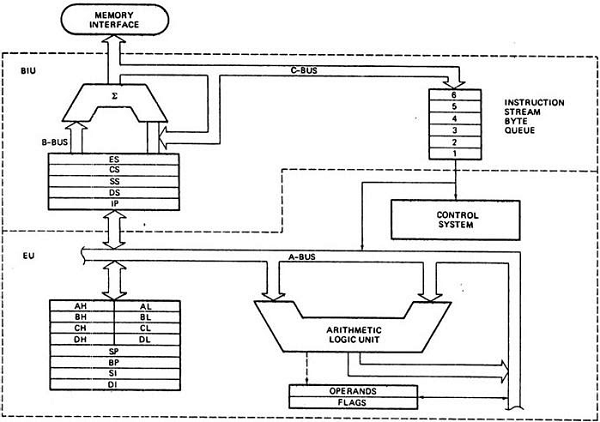
\includegraphics[width=0.65\textwidth]{figures/02_8086_architecture.jpg}
                \caption{Architecture of 8086} \label{fig:8086_architecture}
            \end{center}
        \end{figure}

    \subsection{Address and Data Buses}
    The 8086 CPU has a unidirectional address bus with 20 address lines and a bidirectional data bus with 16 data lines. \cite{buses} The address bus is used to select the desired memory or I/O device by generating a unique address which corresponds to the memory location or the location of I/O device of the system. The data bus is used to transfer data between the CPU and memory and the CPU and I/O devices.\\

    The address bus is denoted as $A_{19}-A_{0}$ (20 lines) and the data bus $D_{15}-D_{0}$ (16 lines). The peripheral devices implemented with the 8086 in this document however consist of 8-bit data bus architectures. The data bus would therefore be multiplexed and more commonly denoted as $D_{7}-D_{0}$ (8 lines).

    \subsection{Control Bus}
    The control bus of 8086 carries control signals which are used to specify the memory and I/O devices. \cite{buses} The bus is bidirectional and assists the CPU in synchronizing control signals to internal devices and external components. It is comprised of interrupt lines, byte enable lines, read/write signals and status lines.

    \subsection{Pinouts}
    Refer to Appendix \ref{appendix:pinouts} for the pinouts of the chip.

    \section{Decoding}

    \subsection{Programming Logic Device - 16L8}

    \subsection{Programming the PLD}

    \newpage
\section{Clock Generator - 8284A}
The 8184A Clock Generator is an ancillary component to the 8086. This system clock is used to synchronize both internal and external operations using an external oscillator. The device is also used for READY and RESET synchronizations and TTL-level peripheral clock signal generation.

        \begin{figure}[h]
            \begin{center}
                
\includegraphics[width=0.4\textwidth]{figures/8284a.png}
                \caption{8284A Clock Generator} \label{fig:8284a}
            \end{center}
        \end{figure}

    \subsection{Clock Speed}
    The 8086 internal clock has a frequency of 5 MHz ($\frac{1}{3}$ of CLK). The external crystal typically oscillates at 15 MHz.

    \subsection{RESET Operation}
    Correct reset timing requires that the RESET input to the 8086 becomes a logic 1 in 4 clock cycles and remain high for at least 50 $\mu S$. The reset switch is implemented in a RC circuit with typical resistance of $100 \ k\Omega$ and $10 \ \mu F$.

    \subsection{Pinouts}
    Refer to Appendix \ref{appendix:pinouts} for the pinouts of the chip.

    \section{Memory Architecture}
The board implemented in this document consists of 128 kB of SRAM and 256 kB of CMOS flash memory.

    \subsection{Static Random Access Memory - CY7C199}
    Static RAM, or SRAM, is a type of volatile memory where bits are stored as long as power is supplied. They are ideal for cache memory because of their fast access times as low as 10 ns. CY7C199 SRAM chips are used to implement the SRAM on this system.

    \subsection{Addressing}
    The SRAM implemented in the system is composed of 32k $\times$ 8 CY7C199 SRAM chips decoded into two banks, with the lowest address at 0x00000.

    \subsection{CMOS Flash Memory - 28F010}
    Flash memory, or electrically erasable programmable ROM (EEPROM), is a type of non-volatile memory which maintains its state even after loss of power. Writing to this memory is much slower than a normal RAM, and it is used to store setup information. 28F010 CMOS chips are used to implement the flash memory on this system.

    \subsection{Addressing Flash Memory}
    The flash memory implemented in the system is composed of 128k $\times$ 8 28F010 CMOS chips decoded into two banks, with the highest address at 0xFFFFF.

    \subsection{Pinouts}
    Refer to Appendix \ref{appendix:pinouts} for the pinouts of the chips.

    \newpage
\section{Programmable Keyboard/Display Interface - 8279}

    \subsection{Description}

    \subsection{Interfacing with a 5x5 Keyboard Matrix}

    \subsection{Addressing}

    \subsection{Programming the Keyboard Interface}

    \subsection{Command Words to Program the 8279}

    \subsection{Assembly Implementation}

    \section{Programmable Interval Timer - 8254}

    \subsection{Programming}

    \subsection{Addressing}

    \subsection{Assembly Implementation}

    \subsection{Pinouts}
    Refer to Appendix \ref{appendix:pinouts} for the pinouts of the chip.

    \newpage
\section{External Headers}

    \subsection{Description}

    \subsection{Interfacing 30-Pin Headers with the 8255}

    \subsection{Addressing}

    \subsection{Assembly Implementation and Programming of the 8255}

    \subsection{Interfacing 14-Pin Headers with the 8254}

    \subsection{Interfacing 14-Pin Headers with the 8259}

    \subsection{Interfacing 60-Pin External Header to the Address, Data and Control Bus}

    \newpage
\section{Interrupt Controller - 8259}

    \subsection{Implementing a Master Interrupt Controller}

    \subsection{Addressing}

    \subsection{Assembly Implementation and Programming}

    \newpage
\section{UART}

    \subsection{16550 UART}

    \subsection{Addressing the 16550}

    \subsection{Programming the 16550}

    \subsection{Assembly Implementation}

    \subsection{MAX-235 and D-SUB-9}

    \subsection{Device Descriptions and Implementations}

    \subsection{Pinouts}
    Refer to Appendix \ref{appendix:pinouts} for the pinouts of the chip.

    \newpage

\section{LCD Display}

    \subsection{Addressing}

    \subsection{Assembly Implementation}
    \newpage

\section{LEDs and DIP Switches}

    \subsection{Seven-Segment LEDs}

    \subsection{Addressing}

    \subsection{LEDs}

    \subsection{Addressing}

    \subsection{DIP Switches}

    \subsection{Addressing}

    \newpage
\appendix
\addcontentsline{toc}{section}{Appendix}

    \section{Appendix A: Schematics}

    \section{Appendix B: Pinouts}

        \label{appendix:pinouts}

        \subsection{8086 Chipset}

                \begin{itemize}

                    \item $M/\overline{IO}$: (Memory/ I/O) indicates if the address is a memory or I/O address

                    \item $\overline{INTA}$: (Interrupt Acknowledgment) generated in response to $INTR$ to put the interrupt vector on the data bus

                    \item $ALE$: (Address Latch Enable) when 1, address data bus contains a memory or I/O address

                    \item $\overline{DEN}$: (Data Bus Enable) activates external data bus buffers

                \end{itemize}


\addcontentsline{toc}{section}{References}
    \begin{thebibliography}{9}

    \bibitem{buses}
    http://gradestack.com/Microprocessors-and/Architecture-of-8086-and/Address-Bus-Data-Bus-/19317-3912-38171-study-wtw

    \end{thebibliography}
    \newpage
\addcontentsline{toc}{section}{References}
    \begin{thebibliography}{9}

    \bibitem{buses} DBHJDS
    http://gradestack.com/Microprocessors-and/Architecture-of-8086-and/Address-Bus-Data-Bus-/19317-3912-38171-study-wtw

    \end{thebibliography}


\end{document}
